\section{Multi-Agent Reinforcement Learning}

% ---------------------------------------------------------------- Thread transition
\begin{frame}{}
\vfill
\centering
{\large Thread 2 of 3}\\[0.5em]
{\LARGE \textbf{Multi-Agent RL}}\\[0.8em]
{\footnotesize\itshape The RLHF deep dive is done. A shorter overview now: what
changes when \emph{other learning agents} share your environment.}
\vfill
\end{frame}

% ================================================================ 4.1
% Why MARL is hard (non-stationarity) - TikZ
\begin{frame}{Why Multi-Agent RL Is Hard: Non-Stationarity}
\centering
\resizebox{0.92\linewidth}{!}{%
\begin{tikzpicture}[font=\footnotesize,
    box/.style={draw, rounded corners, minimum width=2.2cm, minimum height=1.0cm, align=center},
    ar/.style={-{Stealth[length=2.2mm]}, thick}]

  % ---- single-agent ----
  \node[font=\bfseries] at (1.6,3.2) {Single-agent};
  \node[box, fill=sysblue] (a1) at (0,1.6) {Agent};
  \node[box, fill=boxgreen](e1) at (3.2,1.6){Environment\\\scriptsize stationary};
  \draw[ar] (a1.north) to[bend left=35] node[above,font=\scriptsize]{action} (e1.north);
  \draw[ar] (e1.south) to[bend left=35] node[below,font=\scriptsize]{state, reward} (a1.south);

  % divider
  \draw[gray, dashed] (5.4,-0.6) -- (5.4,3.4);

  % ---- multi-agent ----
  \node[font=\bfseries] at (9.5,3.2) {Multi-agent};
  \node[box, fill=sysblue] (a2) at (7.0,1.6) {Agent $i$};
  \node[draw, rounded corners, fill=boxred, align=center, minimum width=3.6cm, minimum height=1.7cm]
        (e2) at (11.0,1.6) {Environment\\\scriptsize \emph{contains other}\\\scriptsize \emph{learning agents}\\\scriptsize non-stationary};
  \draw[ar] (a2.north) to[bend left=25] node[above,font=\scriptsize]{action} (e2.north west);
  \draw[ar] (e2.south west) to[bend left=25] node[below,font=\scriptsize]{state, reward} (a2.south);
\end{tikzpicture}%
}
\vfill
\begin{itemize}\itemsep0.25em\small
    \item Each agent's environment is \textbf{non-stationary}: the others are
          updating their policies at the same time, so the ground shifts as they
          learn; single-agent convergence guarantees break.
    \item Formalized as a \textbf{Markov game} (stochastic game), the multi-agent
          generalization of the MDP.
    \item Three regimes along one axis: \textbf{cooperative} / \textbf{competitive}
          / \textbf{mixed}.
\end{itemize}
\end{frame}

% ================================================================ 4.2
% CTDE - TikZ
\begin{frame}{Centralized Training, Decentralized Execution (CTDE)}
\centering
\resizebox{0.78\linewidth}{!}{%
\begin{tikzpicture}[font=\footnotesize,
    ag/.style={draw, rounded corners, minimum width=1.8cm, minimum height=0.9cm, align=center, fill=sysblue},
    cr/.style={draw, rounded corners, minimum width=4.2cm, minimum height=1.0cm, align=center, fill=boxtan},
    ar/.style={-{Stealth[length=2.2mm]}, thick}]

  % ---- training ----
  \node[font=\bfseries] at (2.2,3.4) {Training (centralized)};
  \node[ag] (t1) at (0.6,1.4) {Actor 1};
  \node[ag] (t2) at (3.4,1.4) {Actor 2};
  \node[cr] (cc) at (2.0,-0.2) {Centralized critic\\\scriptsize sees all obs.\ \& actions};
  \draw[ar] (t1) -- (cc);
  \draw[ar] (t2) -- (cc);
  \draw[ar] (cc.west) to[bend left=20] (t1.south west);
  \draw[ar] (cc.east) to[bend right=20] (t2.south east);

  % divider
  \draw[gray, dashed] (6.0,-0.9) -- (6.0,3.6);

  % ---- execution ----
  \node[font=\bfseries] at (9.8,3.4) {Execution (decentralized)};
  \node[ag] (e1) at (8.2,1.4) {Actor 1};
  \node[ag] (e2) at (11.4,1.4) {Actor 2};
  \node[draw, rounded corners, dashed, gray, minimum width=4.2cm, minimum height=1.0cm,
        align=center] (gone) at (9.8,-0.2) {\textcolor{gray}{critic removed}};
  \node[font=\scriptsize, above=0.05cm of e1] {local obs.};
  \node[font=\scriptsize, above=0.05cm of e2] {local obs.};
\end{tikzpicture}%
}
\vspace{0.4em}
\begin{itemize}\itemsep0.2em\small
    \item \textbf{At training:} a centralized critic sees every agent's
          observations and actions. Because it accounts for what the others did,
          each agent's learning signal becomes \emph{stationary}, defusing the
          non-stationarity problem from the last slide.
    \item \textbf{At execution:} each agent keeps only its \emph{own actor} acting
          on its \emph{local observation}; the critic is gone.
    \item This is the dominant MARL paradigm, the key idea to remember.
\end{itemize}
\end{frame}

% ================================================================ 4.3
% Methods (table)
\begin{frame}{MARL Methods (Named, Not Derived)}
\centering
\renewcommand{\arraystretch}{1.4}
\begin{tabular}{@{}p{3.4cm} p{3.0cm} p{5.0cm}@{}}
\toprule
\textbf{Method} & \textbf{Family} & \textbf{What it solves} \\
\midrule
Independent learners & each runs own DQN & simple baseline; \emph{ignores}
        non-stationarity \\
MADDPG \scriptsize(Lowe 2017) & CTDE actor--critic & centralized critic
        \emph{per agent}; mixed coop/compete \\
VDN / QMIX \scriptsize(2018) & value decomposition & factor a joint value into
        per-agent utilities (QMIX: monotonic mixing) for cooperative tasks \\
\bottomrule
\end{tabular}
\vfill
{\footnotesize The progression: from pretending other agents are part of the
environment, to explicitly modelling the joint value during training.}
\srcnote{\scriptsize Lowe et al.\ 2017 (MADDPG); Sunehag et al.\ 2018 (VDN); Rashid et al.\ 2018 (QMIX).}
\end{frame}

% ================================================================ 4.4
% Self-play (examples carry it - no custom diagram)
\begin{frame}{Self-Play: The MARL Story You Already Know}
\begin{itemize}\itemsep0.4em
    \item An agent improves by \textbf{playing against past versions of itself}:
          \emph{policy $\rightarrow$ plays past versions $\rightarrow$ game data
          $\rightarrow$ improve $\rightarrow$} (repeat).
    \item This creates an \textbf{automatic curriculum}: the opponent gets harder
          exactly as you do, with no hand-designed difficulty schedule.
\end{itemize}
\vfill
\begin{columns}[c]
\begin{column}{0.34\textwidth}
\centering
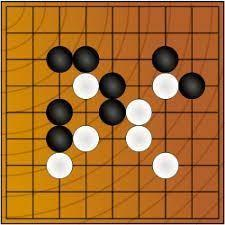
\includegraphics[width=0.9\linewidth,height=0.34\textheight,keepaspectratio]{images/rl-real-world/figures/go.jpg}\\
{\scriptsize \textbf{AlphaGo / AlphaZero}\\(Silver et al.)}
\end{column}
\begin{column}{0.33\textwidth}
\centering
{\scriptsize\textbf{AlphaStar}\\StarCraft II\\(Vinyals et al., 2019)}\\[0.5em]
{\scriptsize\textbf{OpenAI Five}\\Dota 2 (2019)}
\end{column}
\begin{column}{0.33\textwidth}
\centering
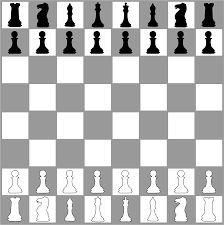
\includegraphics[width=0.9\linewidth,height=0.34\textheight,keepaspectratio]{images/rl-real-world/figures/chess.jpg}\\
{\scriptsize \textbf{Chess} (AlphaZero)}
\end{column}
\end{columns}
\vfill
{\footnotesize \empr{Forward hook:} self-play's automatic curriculum connects to
\textbf{Day 10} (open problems / emergent complexity).}
\end{frame}
